\documentclass[8pt]{beamer}

\usepackage[latin1]{inputenc}
\usepackage[french]{babel}
\usepackage{xcolor}
\usepackage{graphicx}
\usepackage{floatflt}

\title{3dSMin}
\author{Florian Lefevre \& Franck Trey corporation}

\usetheme{Warsaw}
\usecolortheme{seahorse}


\begin{document}

\begin{frame}
	
	\begin{center}
	
\includegraphics[width=11cm]{images/logo.jpg}
	\end{center}
	%\titlepage
\end{frame}

\begin{frame}
	\frametitle{Sommaire}
	\tableofcontents
\end{frame}

\section{Pr�sentation du projet}

	\begin{frame}
		\begin{block}{}
			\begin{center}
				Pr�sentation du projet
			\end{center}
		\end{block}
	\end{frame}

	\begin{frame}
		\frametitle{Objectifs}
		\begin{block}{Objectifs}
			\begin{enumerate}
				\item d�veloppement d'un logiciel de pr�sentation d'objets 3D polygonaux ;
				\item chargement d'objets 3D � partir de fichiers ;
				\item modification de l'angle de vue ;
				\item jeux de lumi�re ;
			\end{enumerate}
		\end{block}
		\begin{block}{Bonus}
			\begin{enumerate}
				\item interface QT ;
				\item gestion du format SFF ;
				\item d�placement de la sc�ne ;
				\item algorithme de rendu ;
				\item sauvegarde des objets 3D ;
				\item gestion de la transparence et des couleurs ;
				\item plusieurs modes d'affichage ;
			\end{enumerate}
		\end{block}
	\end{frame}
		
\section{Etude du projet}

	\begin{frame}
		\begin{block}{}
			\begin{center}
				Etude du projet
			\end{center}
		\end{block}
	\end{frame}

	\subsection{Fichiers ressources}

		\begin{frame}
			\frametitle{Format OFF : structure du fichier}
			\begin{block}{Ent�te}
			\begin{itemize}
				\item code "OFF" ;
				\item nombres de points et nombres de polygones ;
			\end{itemize}
			\end{block}
			\begin{block}{Liste des points}
			\begin{itemize}
				\item coordonn�es (x, y, z) ;
			\end{itemize}
			\end{block}
			\begin{block}{Liste des polygones}
			\begin{itemize}
				\item nombres de points ;
				\item liste des r�f�rences des points ;
				\item informations sur la couleur (composantes r, g, b, $\alpha$ ) ;
			\end{itemize}
			\end{block}
			
		\end{frame}
		
		\begin{frame}
			\frametitle{Format OFF : fichier exemple}
			\begin{block}{exemple.off}
				OFF\newline
				\# commentaire\newline
				8 6 0\newline
				 0.0   1.0   1.0\newline
				 1.0   1.0   0.0\newline
				 0.0   1.0  -1.0\newline
				-1.0   1.0   0.0\newline
				...\newline
				4  0 1 2 3  1.0 0.0 0.0 0.75\newline
				4  7 4 0 3  0.0 1.0 0.0 0.75\newline
				4  4 5 1 0  0.0 0.0 1.0 0.75\newline
				4  5 6 2 1  1.0 0.0 1.0 0.75\newline
				...
			\end{block}
		\end{frame}
		
		\begin{frame}
			\frametitle{Format SFF : structure du fichier}
			\begin{block}{Ent�te}
			\begin{itemize}
				\item code "SFF" ;
				\item nombres d'objets 3d ;
			\end{itemize}
			\end{block}
			\begin{block}{Liste des objets 3d}
			\begin{itemize}
				\item r�f�rence vers le fichier OFF ;
				\item coordonn�es du barycentre de l'objet (x, y, z) ;
				\item facteur de grossissement ;
			\end{itemize}
			\end{block}
			
		\end{frame}
		
		\begin{frame}
			\frametitle{Format SFF : fichier exemple}
			\begin{block}{exemple.sff}
				SFF\newline
				\# commentaire\newline
				2\newline
				../OFF/venus.off			 0.00  0.00  0.00 1.00\newline
				../OFF/nefertiti-entire.off  0.05 -1.99 -0.60 1.50
			\end{block}
			
		\end{frame}
		
	\subsection{Etude de la projection}
	
		\begin{frame}
			\frametitle{Rep�res math�matiques}
			\begin{center}
			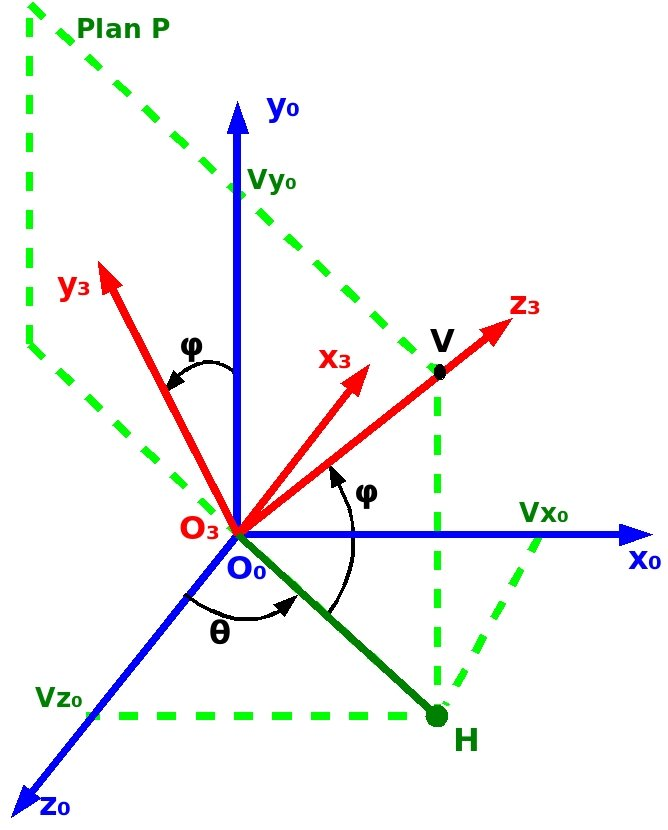
\includegraphics[width=4cm]{images/schema_angle_de_vue.jpg}
			\hspace{1cm}
			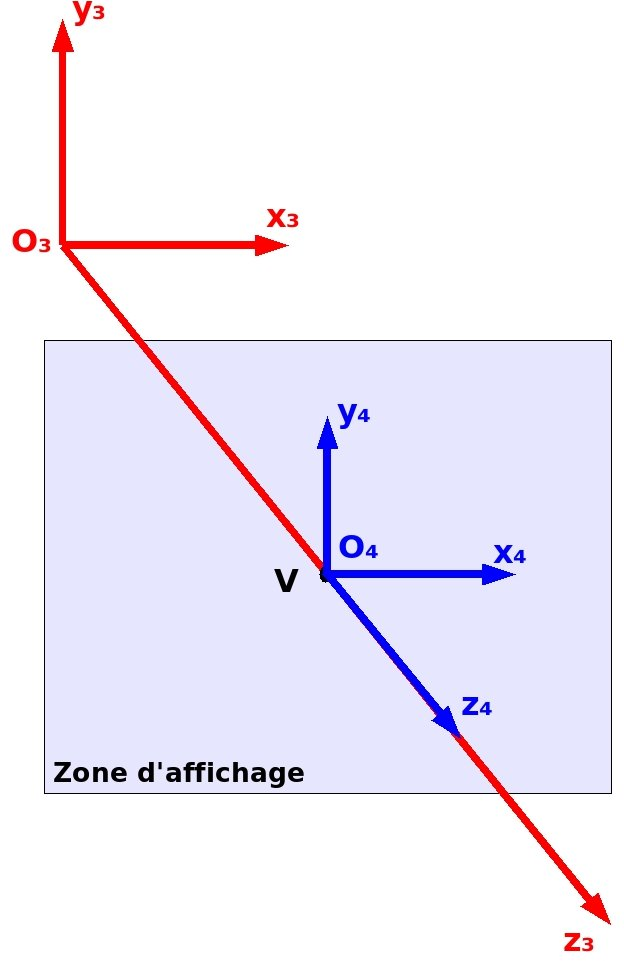
\includegraphics[width=4cm]{images/schema_repere_r3r4.jpg}
			\end{center}
		\end{frame}
		
		\begin{frame}
			\frametitle{Affichage}
			\begin{block}{Rotation selon $\phi$}
				$x_{A_3} = x_{A_0}\cos (\phi)-z_{A_0}\sin (\phi)$\newline
				$y_{A_3} = y_{A_0}$\newline
				$z_{A_3} = z_{A_0}\cos(\phi)+x_{A_0}\sin(\phi)$
			\end{block}
			\begin{block}{Rotation selon $\theta$}
				$x_{A_3} = x_{A_0}$\newline
				$y_{A_3} = y_{A_0}\cos (\theta)-z_{A_0}\sin (\theta)$\newline
				$z_{A_3} = y_{A_0}\cos(\theta)+y_{A_0}\sin(\theta)$
			\end{block}
		\end{frame}
		
		\begin{frame}
			\frametitle{Affichage}
			\begin{block}{Projection � l'�cran}	
				$x_{A_5} = x_{A_3}\frac{P_{fuite}-R_{V_0}}{P_{fuite}-z_{A_3}}$ \newline
				$y_{A_5} = y_{A_3}\frac{P_{fuite}-R_{V_0}}{P_{fuite}-z_{A_3}}$
			\end{block}
			\begin{center}
			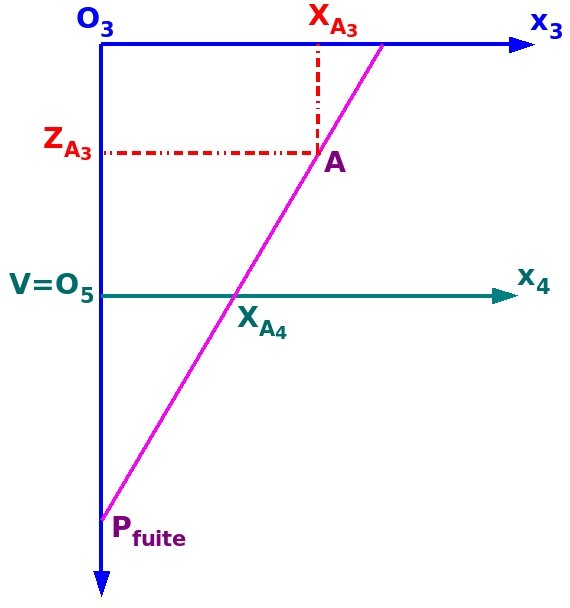
\includegraphics[width=4cm]{images/schema_projection.jpg}
			\end{center}
		\end{frame}
		
	\subsection{Projection de la lumi�re}
	
		\begin{frame}
			\frametitle{Sch�ma d'�tude}
			\begin{center}
			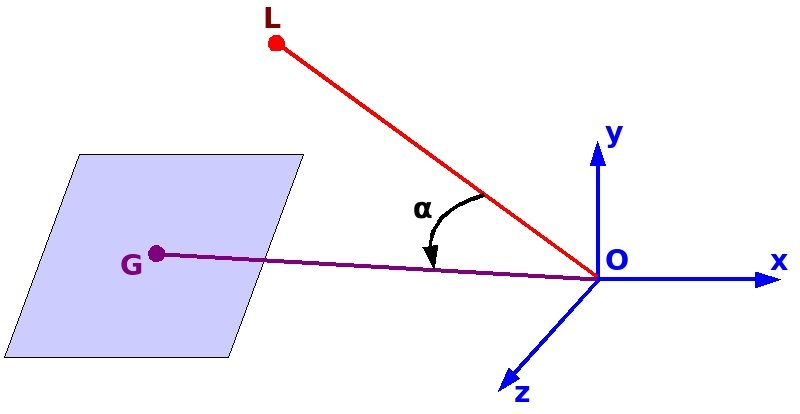
\includegraphics[width=7cm]{images/schema_lumiere.jpg}
			\end{center}
		\end{frame}
		
	\subsection{Interface}
	
		\begin{frame}
			\frametitle{Structuration de l'interface}
			\includegraphics<1>[width=10cm]{images/interface_09.jpg}
			\includegraphics<2>[width=10cm]{images/interface_08.jpg}
			\includegraphics<3>[width=10cm]{images/interface_07.jpg}
			\includegraphics<4>[width=10cm]{images/interface_06.jpg}
			\includegraphics<5>[width=10cm]{images/interface_05.jpg}
			\includegraphics<6>[width=10cm]{images/interface_04.jpg}
			\includegraphics<7>[width=10cm]{images/interface_03.jpg}
			\includegraphics<8>[width=10cm]{images/interface_01.jpg}
		\end{frame}
		
		
\section{Architecture logicielle}

	\begin{frame}
		\begin{block}{}
			\begin{center}
				Architecture logicielle
			\end{center}
		\end{block}
	\end{frame}

	\subsection{Architecture des classes}

		\begin{frame}
			\frametitle{Diagramme des classes}
			\begin{center}
				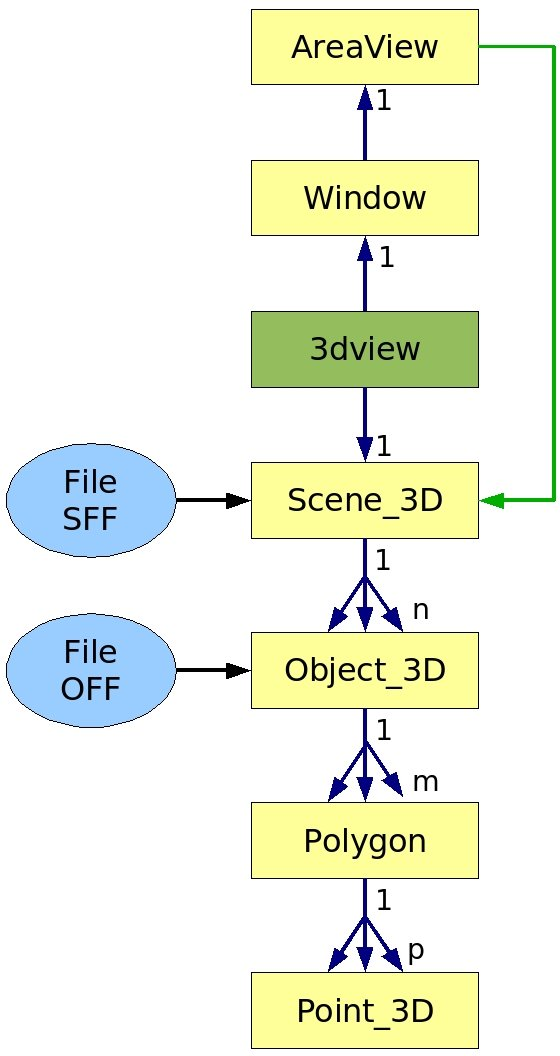
\includegraphics[width=3.5cm]{images/schema_architecture_classe.jpg}
				\hspace{1.5cm}
				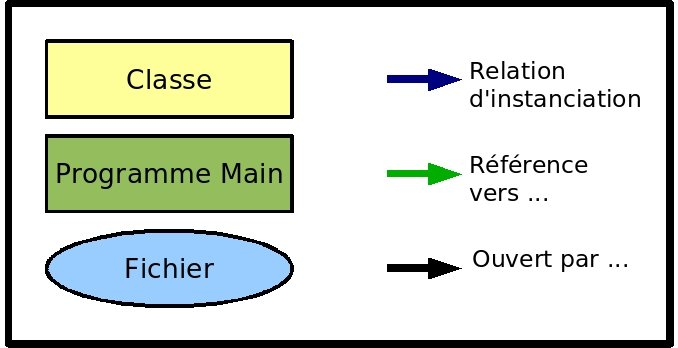
\includegraphics[width=4.5cm]{images/schema_legende_classe.jpg}
			\end{center}
		\end{frame}
		
	\subsection{Algorithmes de rendu}

		\begin{frame}
			\frametitle{Algorithme de lissage}
			\includegraphics<1>[width=10cm]{images/lissage01.jpg}
			\includegraphics<2>[width=10cm]{images/lissage02.jpg}
			\includegraphics<3>[width=10cm]{images/lissage03.jpg}
		\end{frame}
		
		\begin{frame}
			\frametitle{Algorithme de d�coupages}
			\includegraphics<1>[width=10cm]{images/division01.jpg}
			\includegraphics<2>[width=10cm]{images/division02.jpg}
			\includegraphics<3>[width=10cm]{images/division03.jpg}
		\end{frame}
		
	\subsection{Gestion des erreurs}
	
		\begin{frame}
			\frametitle{Interpr�tation des signaux}
			\begin{block}{Principe}
				\begin{itemize}
					\item interception du signal de violation de la m�moire (Seg. Fault.) ;
					\item lib�ration de toutes les instances cr��es ;
					\item aucune erreur de segmentation ;
					\item risque d'instances non d�sallouer ;
					\item processus de fin de programme violent ;
				\end{itemize}
			\end{block}
		\end{frame}
		
\section{Pr�sentation du logiciel}

	\begin{frame}
		\begin{block}{}
			\begin{center}
				Pr�sentation du logiciel
			\end{center}
		\end{block}
	\end{frame}
	
	\subsection{Interface}
	
	\begin{frame}
		\frametitle{Vue globale}
		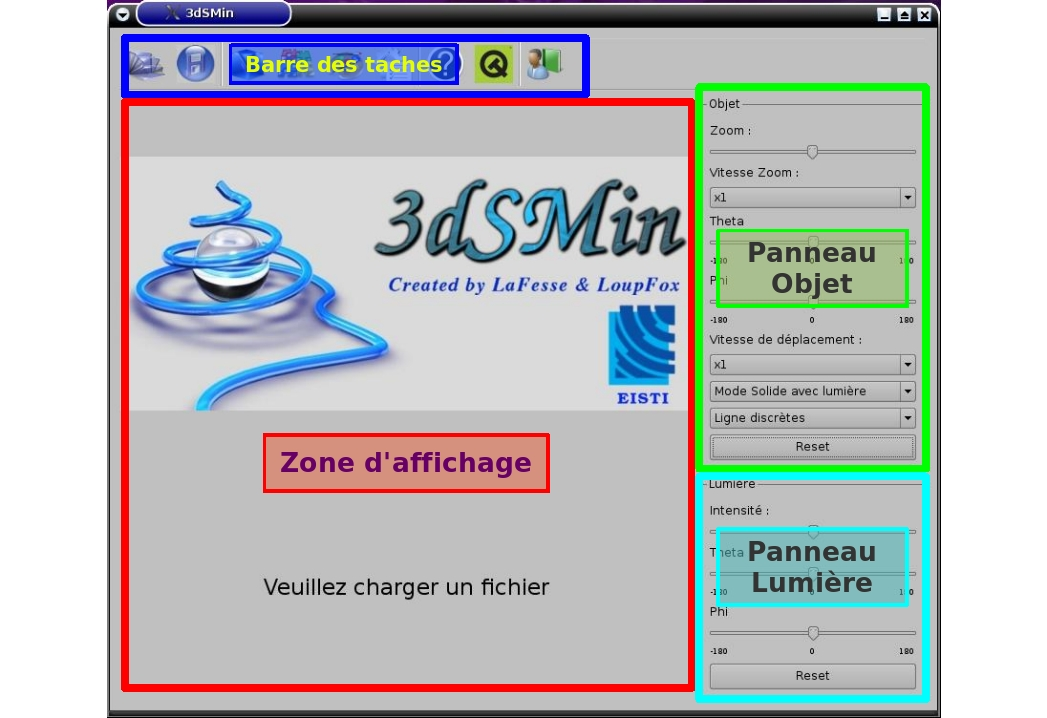
\includegraphics[width=10cm]{images/interface1.jpg}
	\end{frame}
	
	\begin{frame}
		\frametitle{Barre des taches}
		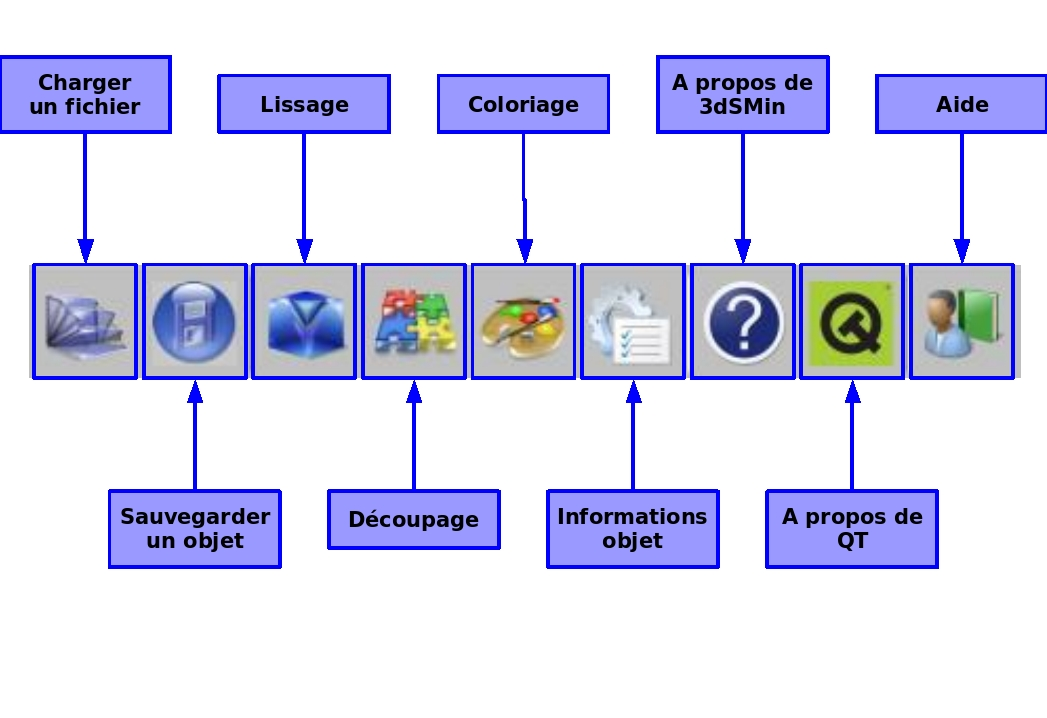
\includegraphics[width=10cm]{images/interface3.jpg}
	\end{frame}
	
	\begin{frame}
		\frametitle{Panneau Objet}
		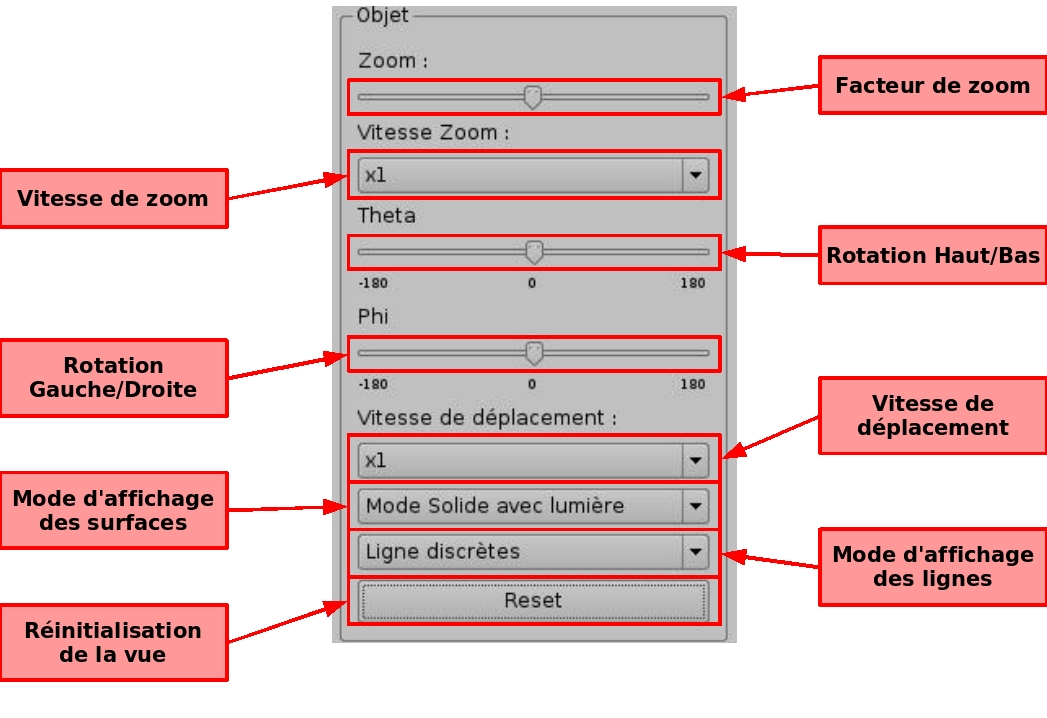
\includegraphics[width=10cm]{images/interface2.jpg}
	\end{frame}
	
	\begin{frame}
		\frametitle{Panneau Lumi�re}
		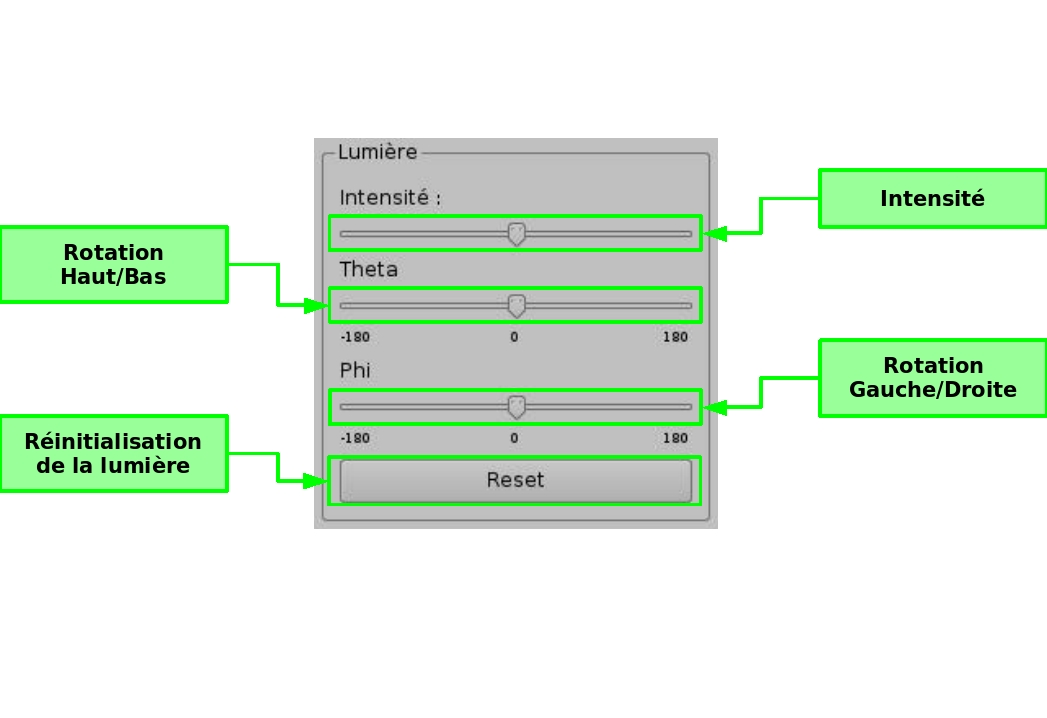
\includegraphics[width=10cm]{images/interface4.jpg}
	\end{frame}
	
	\begin{frame}
		\frametitle{Raccourcis clavier}
		\begin{block}{D�placement de la cam�ra}
			\begin{itemize}
				\item Haut : O / 5 (pav.num.)
				\item Bas : L / 2 (pav.num.)
				\item Gauche : K / 4 (pav.num.)
				\item Droite : M / 6 (pav.num.)
				\item Centrage : C / 5 (pav.num.)
			\end{itemize}
		\end{block}
		\begin{block}{Rotation de la cam�ra}
			\begin{itemize}
				\item Theta (+) : Z / 9 (pav.num.)
				\item Theta (-) : S / 7 (pav.num.)
				\item Phi (+) : D / 3 (pav.num.)
				\item Phi (-) : Q / 1 (pav.num.)
			\end{itemize}
		\end{block}
		\begin{block}{Zoom de la cam�ra}
			\begin{itemize}
				\item Zoom Avant : E / + (pav.num.)
				\item Zoom Arri�re : A / - (pav.num.)
			\end{itemize}
		\end{block}
	\end{frame}

	\begin{frame}
		\begin{block}{}
			\begin{center}
			\textbf{En route vers l'INFINI et l'AU-DELA !!!}
			\end{center}
		\end{block}
		\begin{center}
		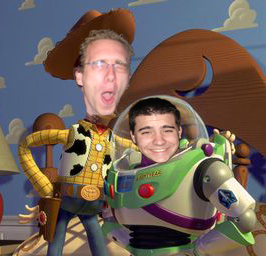
\includegraphics[width=6.5cm]{images/img_fin.jpg}
		\end{center}
		\begin{block}{}
			\begin{center}
			(Sponsored by LaFesse$^{\copyright}$ \& LoupFox$^{\copyright}$ Corporation)
			\end{center}
		\end{block}
	\end{frame}

\end{document}
